% standardmäßig im 4:3 Format
% verwende \documentclass[169]{sikslides} für 16:9
%\documentclass{beamer}
\documentclass{sikslides}
\usepackage{pgfpages}
%\setbeameroption{show notes on second screen}
\graphicspath{{./figures/}}

\title[Speicherkonsistenzmodelle für GPUs]{Speicherkonsistenzmodelle für GPUs}
\subtitle{Seminar \\Safety-Critical Systems}
\author{Marc Blickle}
\date[01.02.2019]{2. Februar 2019}

\begin{document}

\titleframe
\note{\newline \newline Wer von Ihnen hat schonmal was von Cryptocurrency gehört?
\newline \newline Wer von Ihnen hat schonmal was von Bitcoin gehört?
\newline \newline Wer hat Bitcoin besessen oder gemined?
\newline \newline Wer weiß, dass Bitcoin mithilfe von Grafikkarten gemined werden?
\newline \newline
\newline \newline Nicht der einzige Zweck 
\newline \newline Grafikkarten in erster Linie für grafisch Anspruchsvolle Software entwickelt
}



\begin{frame}
	\frametitle{Motivation}
	\begin{itemize}
		\item Vermehrt datenparallele Entwicklung bei GPU
\bigskip
		\item Speicherzugriffe auf Shared Memory müssen abgestimmt sein
\bigskip
		\item Bei CPU etabliert
\bigskip \item GPU-Hersteller hingegen bieten schlechte Transparenz und Info
\bigskip
		\item Datenparallele Entwicklung wird erschwert
	\end{itemize}

\end{frame}
\note{
\new linew Seit einem guten Jahrzehnt wird sich vermehrt auf datenparallele Entwicklung bei GPUs konzentriert
		\newline \newline Parallele Ausführung beudeutet:  Speicherzugriffe auf Shared-Memory müssen vermehrt mithilfe eines sogenannten Speicherkonsistenzmodell abgestimmt werden
\newline \newline Um Fehler zu vermeiden
\newline \newline Bei CPU haben sich Modelle etabliert, 
\newline \newline GPU-Hersteller verwenden zwar auch, bieten aber  schlechte Transparenz, Doku und Info
		\newline \newline Datenparallele Entwicklung wird erschwert
}




\begin{frame}
\frametitle{Speicherkonsistenzmodelle für GPUs}
	    \begin{itemize}
	\item Was sind etablierte CPU-Speicherkonsistenzmodelle?
\bigskip
    \item Wie gut oder schlecht sind sie für den GPU-Gebrauch?
\bigskip
	\item Neue Ansätze?
    \end{itemize}
\end{frame}
\note{\newline \newline Vortrag trägt den Titel Speicherkonsistenzmodelle für GPUs
\newline \newline Möchte folgende Fragen klären
\newline \newline Was sind etablierte CPU-Speicherkonsistenzmodelle?
\newline \newline Wie gut oder schlecht sind sie für den GPU-Gebrauch?
\newline \newline Neue Ansätze?

}

% erneutes Bauen notwendig, um Gliederung zu aktualisieren
\begin{frame}{Gliederung}
   
    \tableofcontents[hideallsubsections]
    	%\tableofcontents[currentsection, subsectionstyle=show/show/hide]
 	%\sectionframe	
	%\subsectionframe
\end{frame}


%\begin{frame}{Motivation}
%  \frametitle{Motivation}
%  \begin{itemize}
%  \item Aufzählungspunkt
%    \begin{itemize}
%    \item Eine Ebene tiefer
%    \item ...


%    \end{itemize}
%  \item Noch ein Punkt
%  \end{itemize}
%\end{frame}
%\sectionframe{Zweiter Teil}


%\begin{frame}
%    \frametitle{Grundlagen}
%    Text ohne Aufzählung
%    \vfill
%    \begin{center}
%        \Large\textbf{Formatierung wie in normale n \LaTeX-Dokumenten möglich}
%    \end{center}
%\end{frame}



\section{Grundlagen}

\begin{frame}{Gliederung}
   
    	\tableofcontents[currentsection, subsectionstyle=show/show/hide]
 	%\sectionframe	
	%\subsectionframe
\end{frame}


\begin{frame}
	\frametitle{Grundlagen}
  \begin{itemize}
  \item GPU-Architektur
\bigskip
  \item Speicherkonsistenz
\bigskip
  \item Speicherkonsistenzmodelle
  \end{itemize}
\end{frame}

%%%GPU ARCHITEKTUR %%%%%%%%%%%%%%%%%%%%%%%%%%%%%%%%%%%
%%UNIT




\begin{frame}
  \frametitle{GPU Architektur - ein Thread}
  \begin{itemize}
  \item Ist eine einzelne Recheneinheit
\bigskip
  \item Führt Rechenoperationen aus
\bigskip
  \item Interagiert mit Speicher
\bigskip
  \item Mehrere tausend Threads 


  \end{itemize}
\end{frame}
\note{ \newline Ein Thread ist eine einzelne Recheneinheit \newline
\newline Führt Rechenoperationen aus, in denen sie mit Speicher interagiert \newline
\newline Tausende Threads können gleichzeitig arbeiten 
} 


%% Block


\begin{frame}
  \frametitle{GPU Architektur - ein Block}
  \begin{itemize}
  \item Mehrere Threads sind in einem Block zusammengefasst
\bigskip
  \item Anzahl unterscheidet sich von Architektur zu Architektur
\bigskip
  \item Parallele und oder serielle Ausführung
\bigskip
  \item Threads in einem Block teilen Shared Memory
\bigskip
  \item Zum Schreiben und Lesen: Über Shared Memory kommunizieren die Threads 
  \end{itemize}
\end{frame}
\note{\newline\newline Mehrere Threads bilden einen Block\newline
\newline Anzahl Je nach Architektur unterschiedlich \newline
\newline Bis zu 512 Threads pro Block \newline
\newline Parallel oder seriell zueinander \newline
\newline Abhängig von Speichermodell \newline
\newline Mehr dazu gleich \newline
\newline Alle Threads im Block teilen sich shared memory \newline
\newline in ihn wird gelesen und geschrieben. \newline
\newline Kommunikation über Shared Memory}


\begin{frame}
	\frametitle{GPU Architektur - ein Block}
\begin{figure}[htbp] 
  \centering
  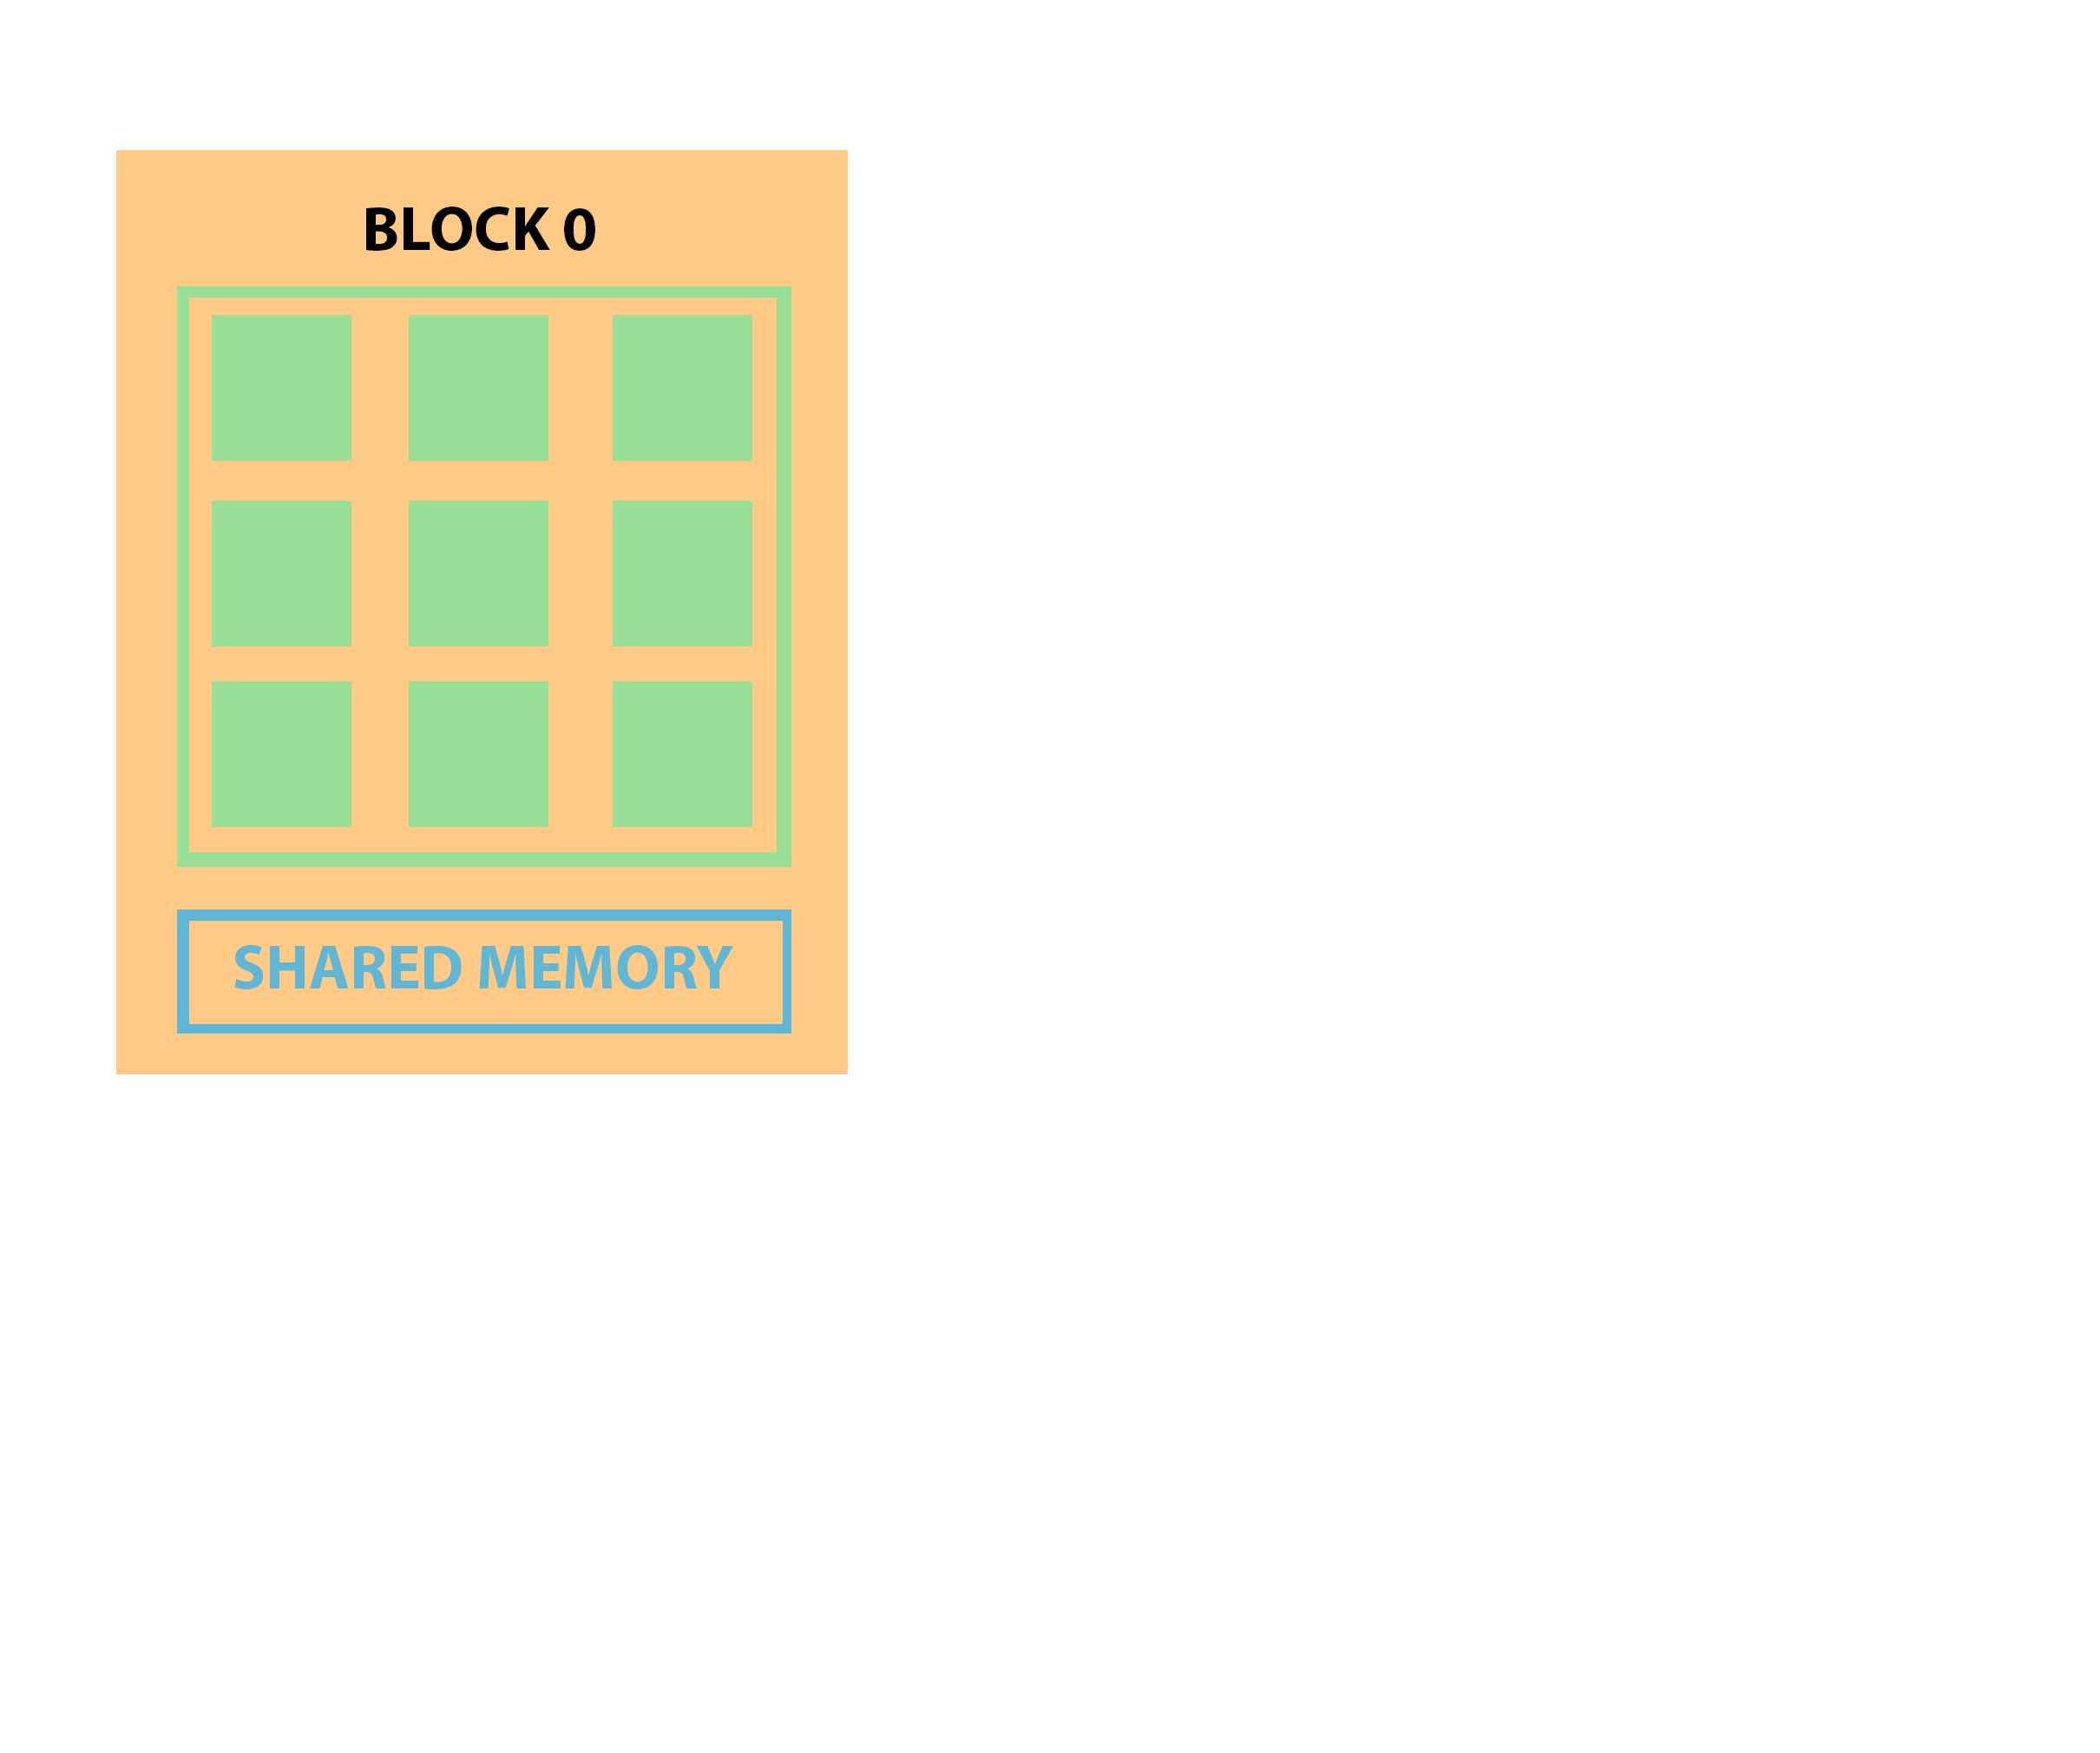
\includegraphics[width=0.9\textwidth]{figures/gpumemory3.png}
  \label{Fig:gpum}
\end{figure}
\end{frame}




%%%Giter

\begin{frame}
	\frametitle{GPU Architektur}
\begin{figure}[htbp] 
  \centering
  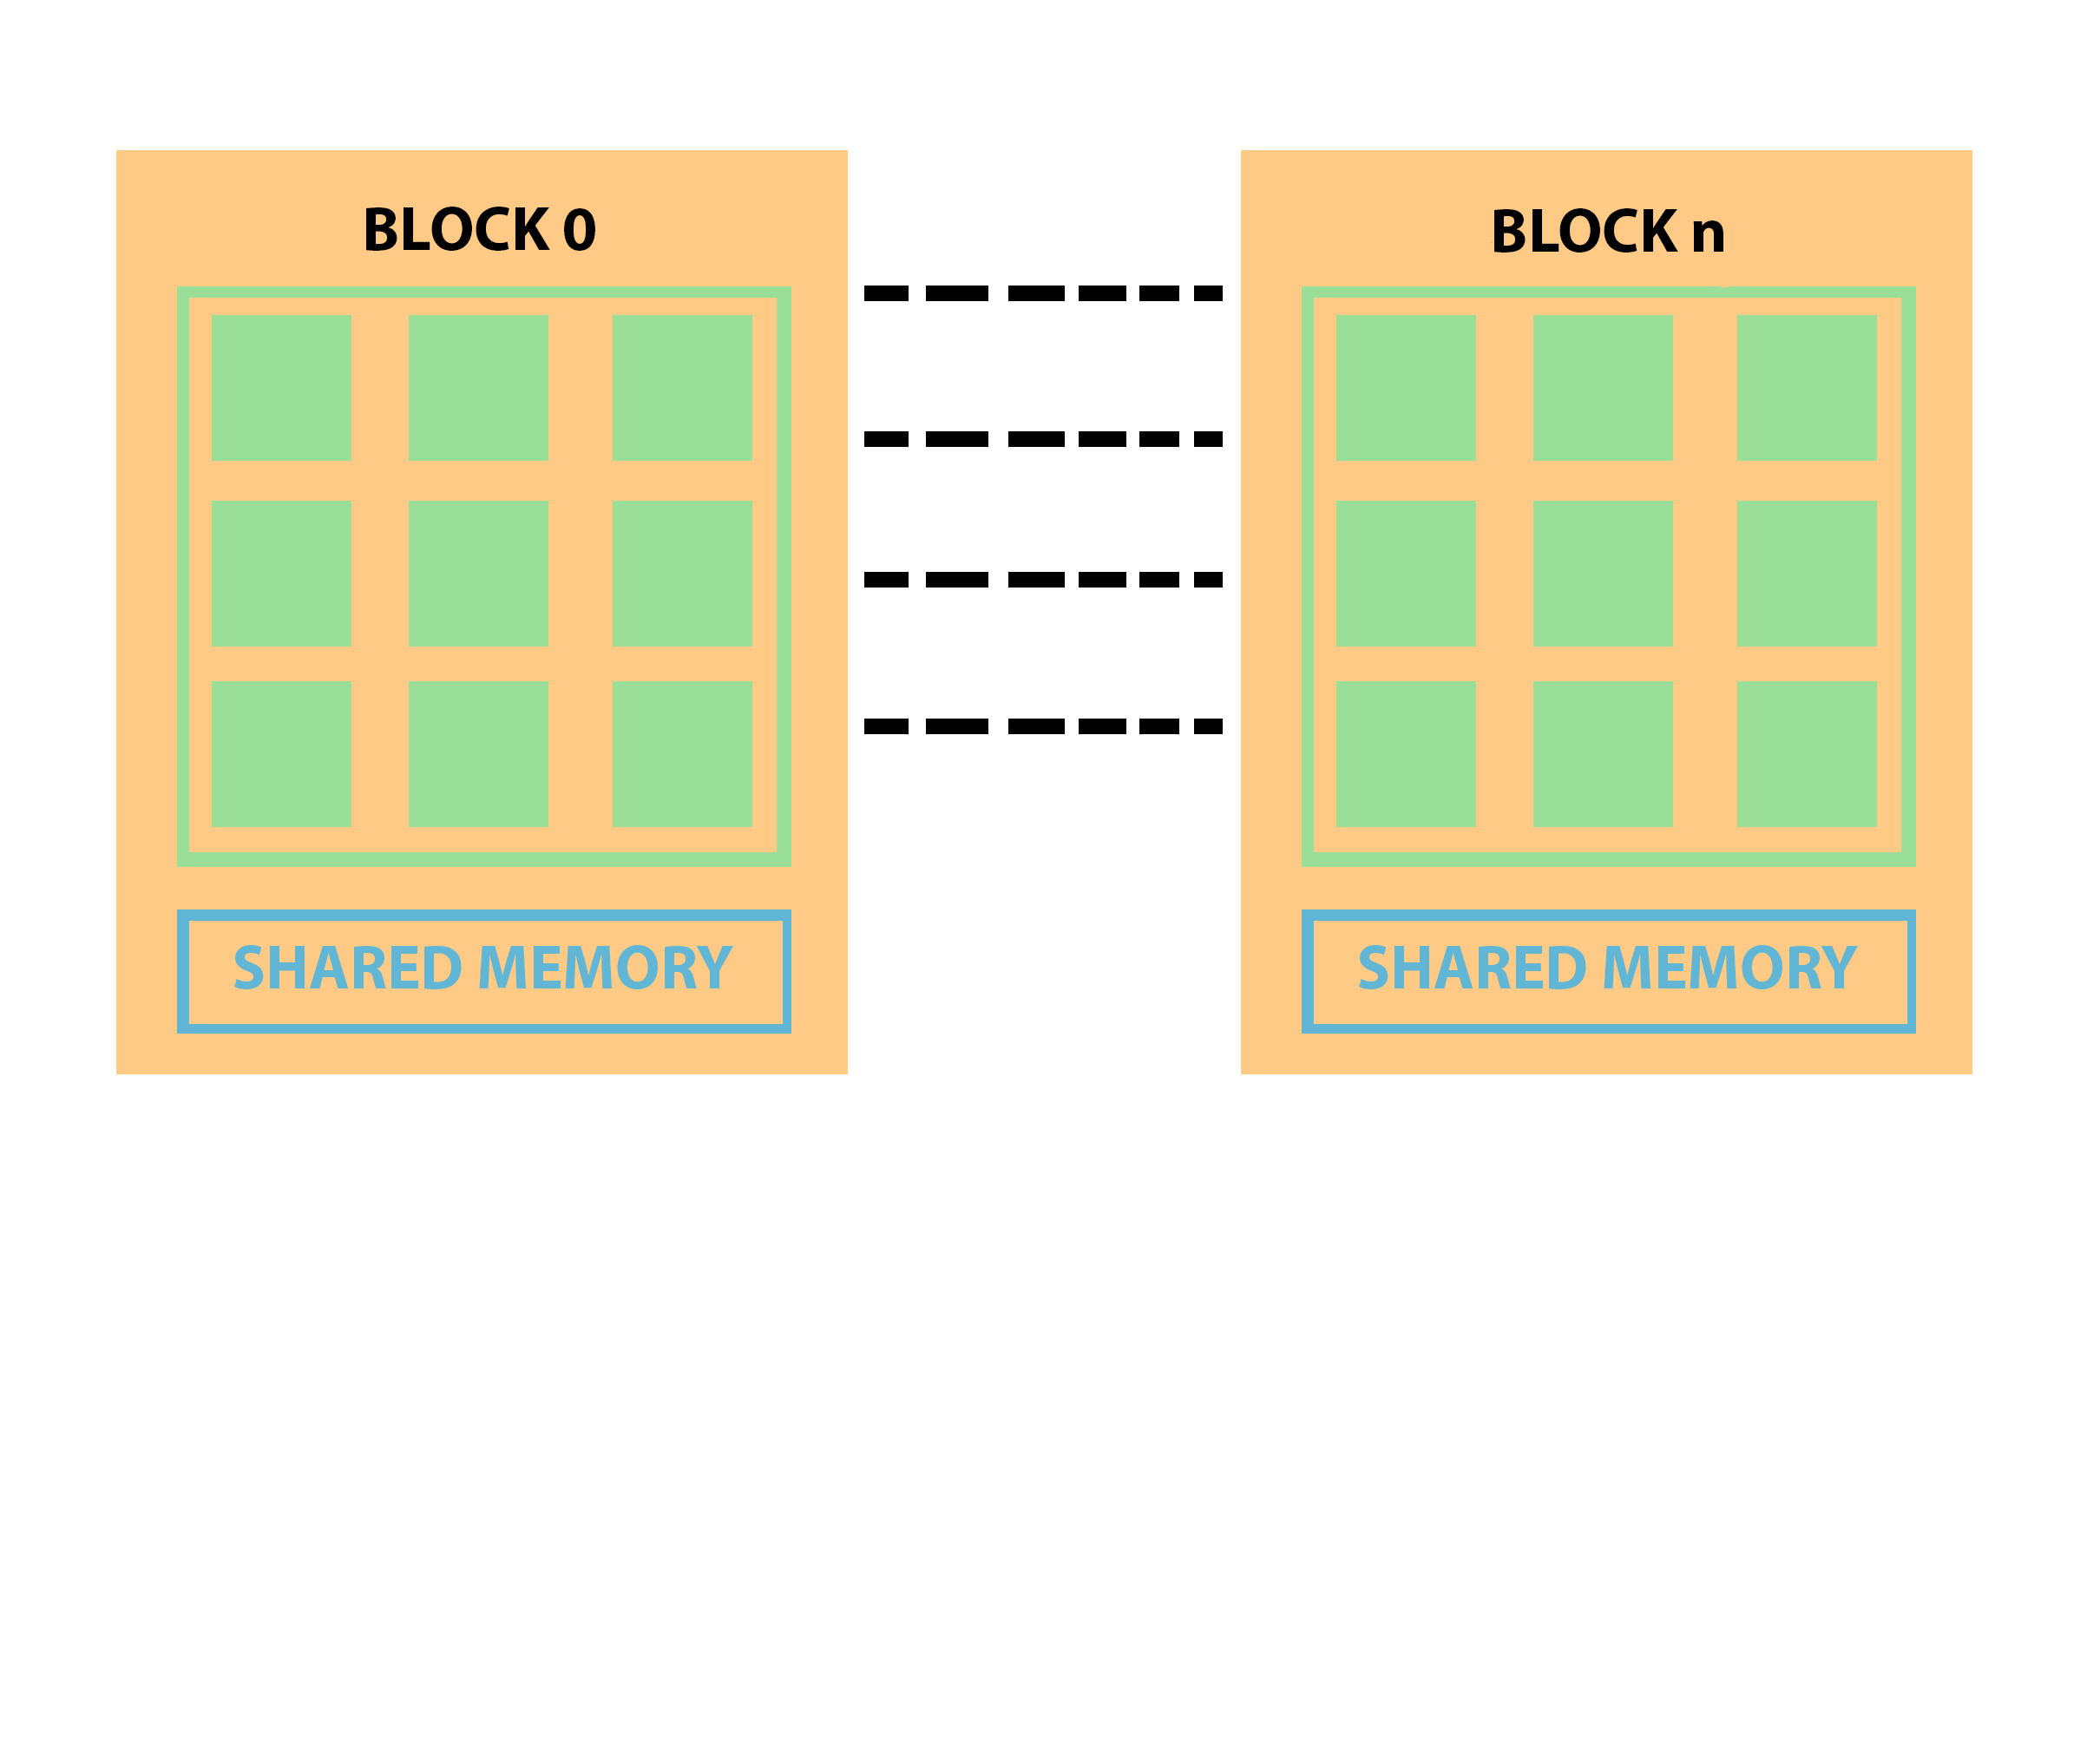
\includegraphics[width=0.9\textwidth]{figures/gpumemory4.png}
  \label{Fig:gpum}
\end{figure}

\end{frame}
\note{ \newline Mehrere Blöcke bilden ein Gitter
\newline \newline  Global Memory steht gesamten Gitter zur Verfügung
\newline \newline Einzelne Blöcke und somit auch die Threads greifen auf ihn zu und kommunizieren über ihn
}

\begin{frame}
	\frametitle{GPU Architektur}
	\begin{figure}[htbp] 
 	 	\centering
 		 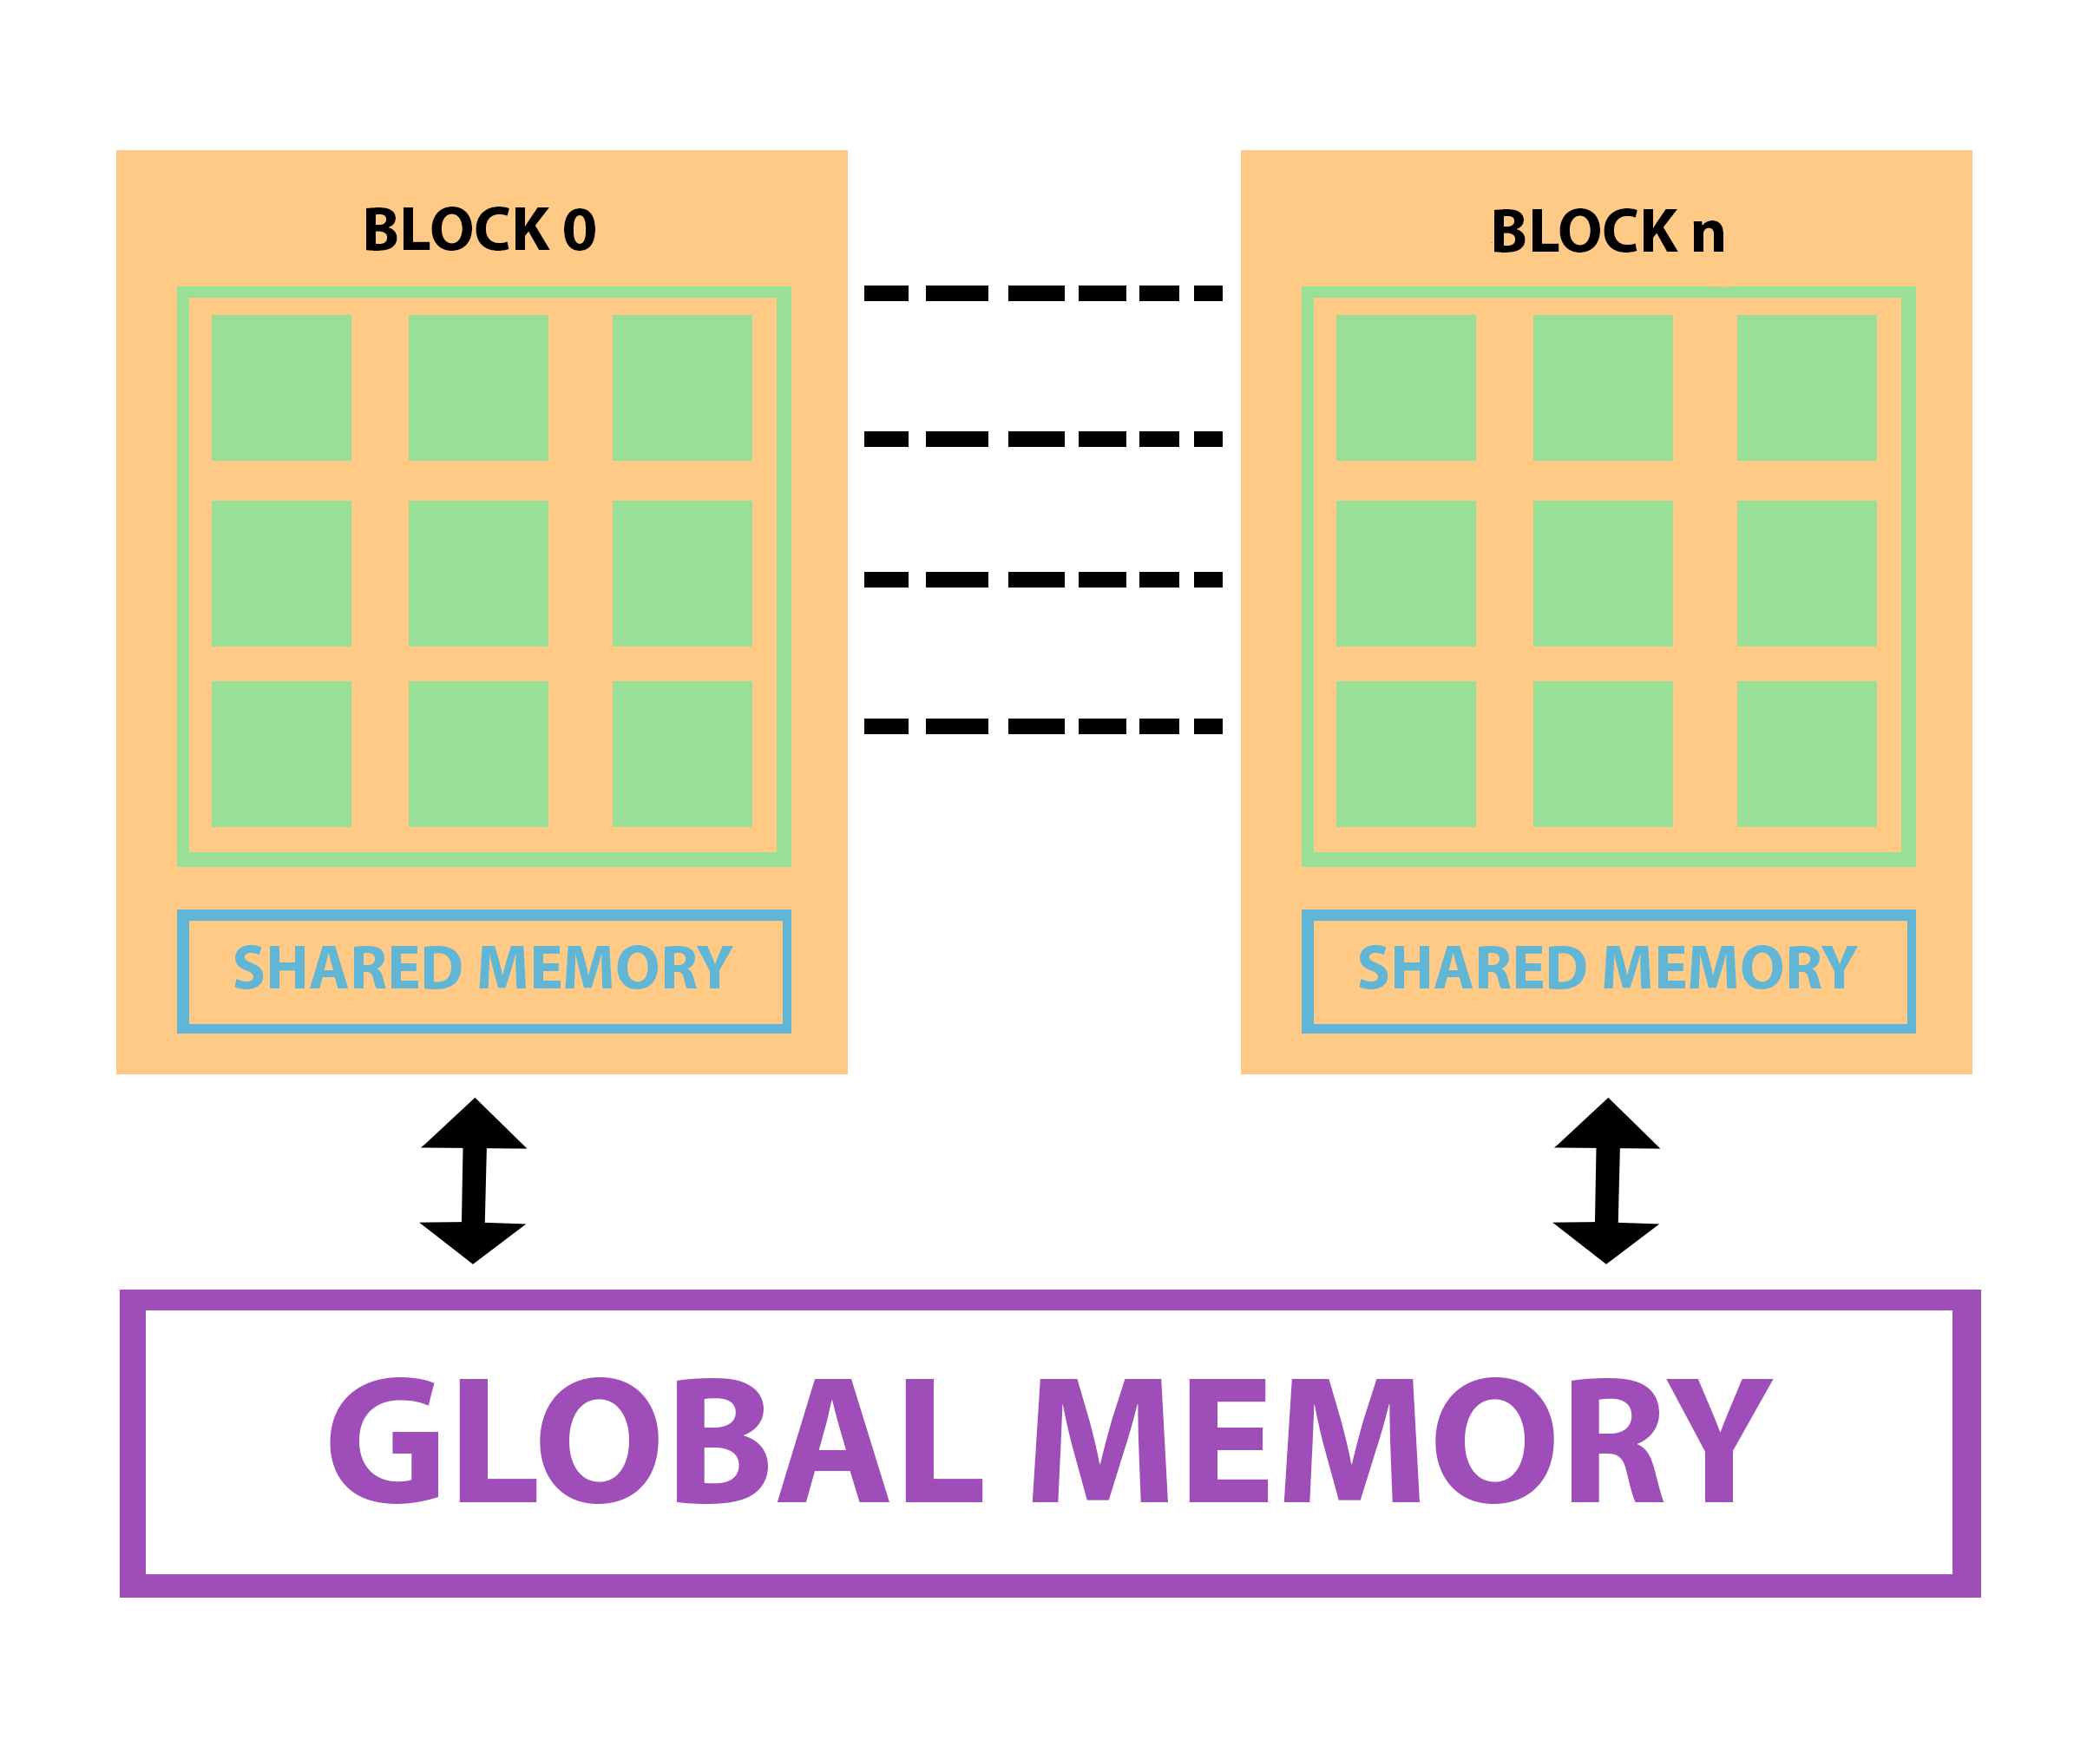
\includegraphics[width=0.9\textwidth]{figures/gpumemory.png}
 		 \label{Fig:gpum}
	\end{figure}

\end{frame}
\note{ \newline Mehrere Blöcke bilden ein Gitter
\newline \newline  Global Memory steht gesamten Gitter zur Verfügung
\newline \newline Einzelne Blöcke und somit auch die Threads greifen auf ihn zu und kommunizieren über ihn
}





\begin{frame}
  \frametitle{GPU Architektur }
	\begin{itemize}
		\item Programmierer entscheidet über Thread- und Blockzahl
\bigskip
		\item Obergrenze allerdings von GPU vorgegeben
\bigskip
		\item Wichtig dabei: Threads müssen Speicherzugriffregeln einhalten
	\end{itemize}
\end{frame}
\note{
\newline  \newline   Wie Units, Blöcke und Gitter gebildet werden, hängt von der laufenden Software ab
\newline  \newline  Verschiedene GPUs, verschiedene architekturen, verschiedene Obergrenzen
\newline  \newline  Bei Softwareprogrammierung zu beachten:
\newline  \newline  Threads Speicherzugriffsregeln einhalten
\newline  \newline es braucht Regelung, wie Threads auf gleichen Speicher zugreifen
\newline  \newline  ohne sich zu behindern
\newline  \newline  Es muss Speicherkonsistenz geschaffen werden
}



%%%%%%%%%%%%% ENDE ARCHITEKTUR %%%%%%%%%%%%%%%%%%%%%%%

%%%%%%%%%%%%%%%%%%%%%%%%%%%%%%%%%SPEICHERKONSISTENZ %%%%%%
\begin{frame}
	\frametitle{Speicherkonsistenz}
Speicherkonsistenz und Speicherkonsistenzmodelle
\end{frame}

\begin{frame}
	\frametitle{Speicherkonsistenz}
	\begin{itemize}
		\item Threads greifen also gemeinsam auf Shared Memory zu
\bigskip
		\item Was passiert, wenn mehrere Threads auf selbe Speicheradresse zugreifen wollen?
	\end{itemize}
\end{frame}
\note{\newline \newline  Threads greifen also gemeinsam auf Shared Memory zu

\newline \newline Was passiert, wenn mehrere Threads auf selbe Speicheradresse zugreifen wollen?}


\begin{frame}
\frametitle{Speicherkonsistenz}
	\begin{figure}[htbp] 
  \centering
  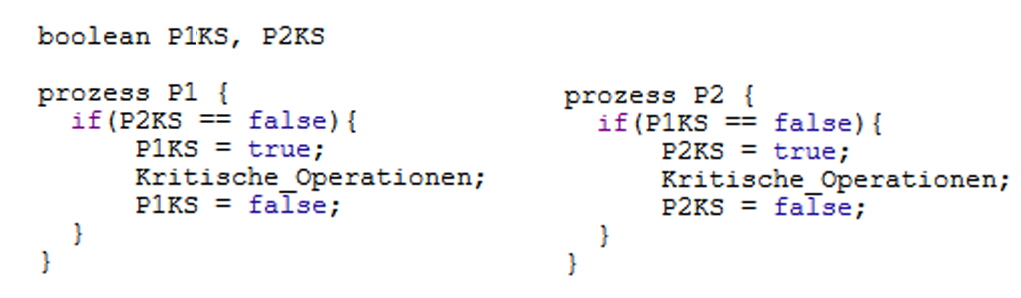
\includegraphics[width=0.9\textwidth]{figures/problem1.png}
  \label{Fig:gpum}
\end{figure}
\end{frame}

\begin{frame}
\frametitle{Speicherkonsistenz}
	\begin{figure}[htbp] 
  \centering
  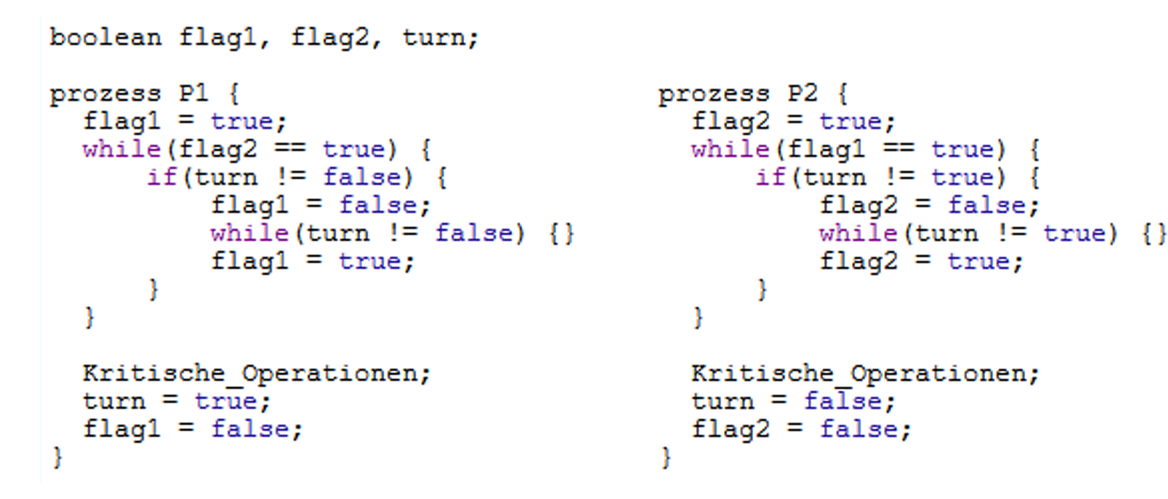
\includegraphics[width=0.9\textwidth]{figures/problem2.png}
  \label{Fig:gpum}
\end{figure}
\end{frame}


\begin{frame}
	\frametitle{Speicherkonsistenz}
	\begin{itemize}
		\item Speicherdaten im System sollen einheitlich und widerspruchfrei sein
\bigskip
		\item Es werden Anforderungen geschaffen, die erfüllt werden müssen um dies zu erreichen
\bigskip
		\item Diese bestimmen, was eine Operation sehen und machen darf
\bigskip
		\item Verschiedene Architekturen bieten verschiedene Anforderungen: verschiedene Speicherkonsistenzmodelle
	\end{itemize}
\end{frame}
\note{\newline \newline Speicherdaten sollen einheitlich und widerspruchfrei sein
\newline \newline Verhindern, dass Speicherfehler entstehen
\newline \newline Hierzu Anforderungen schaffen, die erfüllt werden müssen
\newline \newline Sie bestimmen, was eine Speicheroperation sehen und machen darf
\newline \newline Verschiedene Architekturen 
\newline \newline Verschiedene Anforderungen
\newline \newline Verschiedene Speicherkonsistenzmodelle
}


%%%%%%%%%%%%%%%%%%%%%%%%%%%%%%%%%%%%%%% SPEICHERKONSISTENZMODELLE




\begin{frame}
	\frametitle{Speicherkonsistenzmodelle}
	\begin{itemize}
		\item Modell stellt Vertrag zwischen Software und Speicherhardware dar
\bigskip
		\item Regelwerk, wie das System Speicheroperationen verarbeitet
\bigskip
		\item Bei Einhaltung werden Ergebnisse zugesichert und konsistente Ziele erreicht
\bigskip
		\item Es herrscht dann Speicherkonsistenz
\bigskip
		\item Verschiedene Modelle -  verschiedene Strukturen - verschiedene Zwecke
	\end{itemize}
\end{frame}
\note{\newline \newline Speicherkonsistenzmodell ist Vertrag zwischen Software und Speicher
\newline \newline also Regelwerk, das bestimmt, wie Speicheroperationen ausgeführt werden
\newline \newline Wenn Programmierer und Software es einhalten, kann man mit gewünschten Ergebnissen rechnen
\newline \newline SpeicherKonsistenz ist gewährt
\newline \newline Verschiedene Speicherkonsistenzmodelle
\newline \newline Verschiedene Strukturen
\newline \newline Können für verschiedene Zwecke verwendet werden
}


\begin{frame}
\frametitle{Speicherkonsistenzmodelle}
	Welches Modell ist nun gut für eine GPU?
\end{frame}
\note{\newline \newline Welches für CPU konzipierte Speichermodell ist jetzt gut für GPU?}

\begin{frame}
	\frametitle{Welches Modell ist nun gut für eine GPU?}
	\begin{itemize}
		\item GPU sehr viele Recheneinheiten
		\item GPU verfügt über tieferen Aufbau
\bigskip
		\item Sehr viele parallele Ausführungen
	\end{itemize}
	\bigskip
	$\rightarrow$ GPU braucht Schnelligkeit und Performance, viele Berechnungen
	\newline 
\bigskip
$\rightarrow$  Speicher soll geregelt beschrieben und gelesen werden
\newline
\bigskip
$\rightarrow$  Aber Threads sollen dies schnell und ungehindert tun
\end{frame}

\note{
\newline \newline GPU sehr viele Recheneinheiten
\newline \newline GPU mit Speicherarchitektur auf mehreren Leveln
\newline \newline Mehr parallele Ausführungen, Threads müssen zusammenarbeiten
\newline \newline GPU muss wegen dieser vielen kleinen Operationen schnell sein
\newline \newline Modell muss auf Performance ausgelegt sein
\newline \newline Speicher soll trotzdem geregelt beschrieben und gelesen werden
\newline \newline Ohne Threads zu blockieren
}



\section{Untersuchte Speicherkonsistenzmodelle}
\begin{frame}{Gliederung}
   
    	\tableofcontents[currentsection, subsectionstyle=show/show/hide]
 	%\sectionframe	
	%\subsectionframe
\end{frame}



\begin{frame}
	\frametitle{Untersuchte Speicherkonsistenzmodelle}
  \begin{itemize}
  \item Sequential Consistency Model
\bigskip
  \item Weak Consistency Model
\bigskip
  \item Release Consistency Model
  \end{itemize}
\end{frame}
%%%%%%%%%%%%%%%%%%%%%%%%%%%%%%				SEQUENTIELL
\begin{frame}
	\frametitle{Sequential Consistency Model}
Sequential Consistency Model
\end{frame}




\begin{frame}
	\frametitle{Sequential Consistency Model}
Abstrakt:
	\begin{itemize}
		\item Alle Threads über Switch an gemeinsamen Speicher gekoppelt
\bigskip
		\item Switch gibt Speicher für bestimmten Prozessor frei
\bigskip
		\item Dieser darf nun operieren, meldet wenn fertig
\bigskip
		\item Switch sortiert also die Lese und Schreiboperationen und stellt sequentielle Reihenfolge her
\bigskip
		\item Unabhängig davon, wann sie eingereicht werden, sortiert Switch sinnvoll 
\bigskip
		\item Alle Prozessoren sehen somit dieselbe Reihenfolge
	\end{itemize}
\end{frame}
\note{
\newline \newline Abstrahierung
\newline \newline Alle Threads über Switch an SharedMemory gekoppelt
\newline \newline Threads reichen Operationen ein
\newline \newline Switch gibt gesamten Speicher für einen Prozessor frei
\newline \newline Dieser operiert, meldet wenn fertig
\newline \newline Switch sortiert also alle eingehenden Lese und Schreiboperationen und stellt sinnvolle, sequentielle Reihnefolge her
\newline \newline Für alle Prozessoren gilt nun dieselbe Reihenfolge
}


\begin{frame}
	\frametitle{Sequential Consistency Model}
\begin{figure}[htbp] 
  \centering
  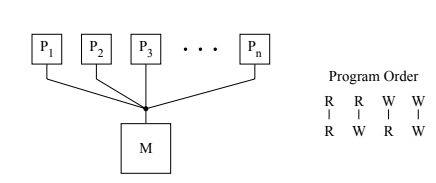
\includegraphics[width=0.9\textwidth]{figures/seqq.PNG}
  \label{Fig:gpum}
\end{figure}
\end{frame}







\begin{frame}
	\frametitle{Sequential Consistency Model}
	Konsistenz resultiert aus Programm, wenn:
\bigskip
	\begin{itemize}
		\item Jeder Prozessor Speicheranfragen in der Reihenfolge einreicht, die Programm vorgibt
\bigskip
		\item Speicheranfragen jedes Prozessors von Schlange verarbeitet werden, die die Anfragen sortiert
	\end{itemize}
\bigskip Globale Reihenfolge für alle eingereichten Operationen!
\end{frame}
\note{
\newline \newline Ein Programm, das unter diesem Regelwerk agiert, stellt eine Konsistenz sicher,
\newline \newline Jeder Prozessor Speicheranfragen in der Reihenfolge einreicht, die ihm vom Programm vorgegeben wurde
\newline \newline Speicheranfragen jedes Prozessors von Schlange verarbeitet werden, die die Anfragen sortiert
\newline \newline Für alle eingereichten Operationen wird eine globale Reihenfolge gewählt, die eingehalten werden muss.
}


\begin{frame}
	\frametitle{Sequential Consistency Model}
\begin{figure}[htbp] 
  \centering
  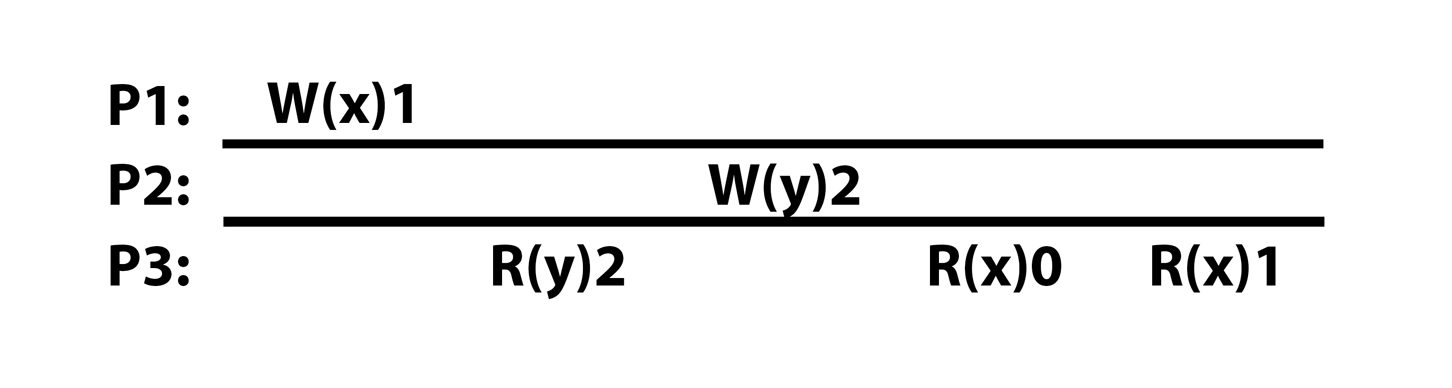
\includegraphics[width=0.9\textwidth]{figures/SeqModell1.PNG}
  \label{Fig:gpum}
\end{figure}
\end{frame}
\note{
\newline \newline PRzessor 3 soll Wert erfassen, der nicht existiert
\newline \newline Der wird erst von Prozessor 2 geschrieben
\newline \newline Eigentlich nicht möglich, wegen Compilererror
\newline \newline Aber zeigt Flexibilität
\newline \newline Switch würde nämlich neu anordnen
}





\begin{frame}
	\frametitle{Sequential Consistency Model}
	Vorteile:
	\begin{itemize}
		\item Ablauf ähnelt stark der Denkweise eines Programmierers\bigskip
	\end{itemize}

	Nachteile:
	\begin{itemize}
		\item Leider ist dieser nicht parallel\bigskip
		\item Modell passt nicht wirklich zu Multiprozessorsystem\bigskip
		\item Sequentielle Abfolge verlangsamt die Ausführung\bigskip
		\item Je mehr Prozessoren, desto schlechter für GPU\bigskip
		\item Prozessoren müssen immer aufeinander warten
	\end{itemize}
\bigskip
\end{frame}
\note{
\newline \newline Vorteile:
\newline \newline Ablauf ähnelt stark der Denkweise eines Programmierers
\newline \newline Ist sequentiell und einfach
\newline \newline Nachteile:
\newline \newline Leider ist dieser nicht parallel
\newline \newline Modell passt nicht wirklich zu Multiprozessorsystem
\newline \newline Sequentielle Abfolge verlangsamt die Ausführung
\newline \newline Je mehr Prozessoren, desto schlechter für GPU
\newline \newline Prozessoren müssen immer aufeinander warten
}



%%%%%%%%%%%%%%%%%%%%%%%%%%%%%%		 		SCHWACH
\begin{frame}
	\frametitle{Weak Consistency Model}
Schwaches Speicherkonsistenzmodell
\end{frame}


\begin{frame}
	\frametitle{Weak Consistency Model}
	\begin{itemize}
		\item Zu dem Zweck entwickelt, Speicherlatenz zu verringern \bigskip
		\item Weiterentwicklung aus sequentiellem Modell \bigskip
		\item Leistungssteigerung von 40\% \bigskip
		
	\end{itemize}
\end{frame}
\note{\newline Zweck: Speicherlatenz verringern (Zeit zischen Anfrage und Erhalt des Wertes vom Prozessor)
\newline \newline Sequentielles Modell so weiterentwickelt, dass zeitweise inkonsistente Modi möglich sind

\newline \newline  40\% mehr Leistung
\newline \newline Softwareentwickler muss die Speicheroperationen genau anpassen
\newline \newline Wir werden gleich noch sehen wieso
}









\begin{frame}
	\frametitle{Weak Consistency Model}
	\begin{itemize}
		\item Datenoperationen: \bigskip
		\begin{itemize}
			\item Werte werden aus Speicher gelesen oder geschrieben \bigskip
			\item Diese Operationen dürfen parallel zueinander ablaufen \bigskip
		\end{itemize}
		\item Deshalb Synchronisationsoperationen: \bigskip
			\begin{itemize}
			\item Bringt Shared Memory auf einen Stand \bigskip
			\item Jeder Prozessor kann diese auslösen \bigskip
			\item Keine neuen Operationen dürfen dann begonnen und laufende müssen abgeschlossen werden \bigskip
			\item Synchronisation ist auch Neuanordnung von laufenden Operationen \bigskip
			\item Optimale Reihenfolge generieren und Performance steigern
			\end{itemize}
	\end{itemize}
\end{frame}
\note{\newline \newline Werte werden aus Speicher gelesen oder geschrieben
\newline \newline Diese Operationen dürfen parallel zueinander ablaufen
\newline \newline  Deshalb Synchronisationsoperationen:
\newline \newline Bringt Shared Memory auf einen Stand
\newline \newline Jeder Prozessor kann diese auslösen
\newline \newline Keine neuen Operationen dürfen dann begonnen und laufende müssen abgeschlossen werden
\newline \newline Synchronisation ist auch Neuanordnung von laufenden Operationen
\newline \newline Optimale Reihenfolge generieren und Performance steigern

}


\begin{frame}
	\frametitle{Weak Consistency Model}
\begin{figure}[htbp] 
  \centering
  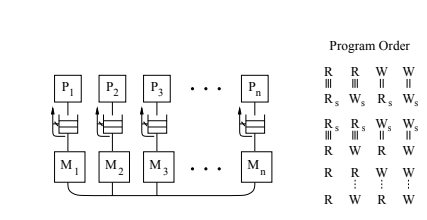
\includegraphics[width=0.9\textwidth]{figures/weeeea.png}
  \label{Fig:weak}
\end{figure}

\end{frame}
\note{ \newline Jeder Prozess kann selber auf Memory zugreifen, 
\newline \newline  Parallel zu den anderen Prozessen
\newline \newline Zwei und Drei Linien: Operation muss abgeschlossen werden, bevor nächste folgen kann
\newline \newline Betrifft ausschließlich Synchronisationsoperationen
\newline \newline Read und Read sind unabhängig voneinander
\newline \newline Gestrichelt: Darf alles parallel ablaufen, außer es betrifft dieselbe Speicheradresse
\newline \newline Führt dazu, dass die Synchronisationsoperationen sequentiell sein müssen, die Datenoperationen aber freier sind
}



\begin{frame}
	\frametitle{Weak Consistency Model}
 Schwache Konsistenz ist gegeben, wenn: \bigskip
	\begin{itemize}
		\item Wenn die Synchronisationsoperationen untereinander sequentiell konsistent sind \bigskip
		\item Alle anderen Operation können in beliebiger Reihenfolge gesehen werden \bigskip
		\item Alle Prozessoren stets alle Synchronisationsoperationen in gleicher sequentieller Reihenfolge sehen 
	\end{itemize}
\end{frame}
\note{
\newline\newline (VON FOLIE ABLESEN)
\newline\newline Um diese Bedingungen realisieren zukönnen, ist jede Recheneinheit dazu in der Lage, 2 Arten von Operationen auszuführen
\newline \newline Gewöhnliche Datenoperationen
\newline \newline Synchronisationsoperationen

}






%%% EVTL BEISPIEL ZEIGEN

\begin{frame}
	\frametitle{Weak Consistency Model}
Vorteile:
	\begin{itemize}
		\item Einzelne Threads können sich in beliebiger Reihenfolge Zugriff verschaffen
		\item Müssen nicht auf andere Prozesse warten
		\item Speicherlatenz wird verringert, Performance gesteigert
	\end{itemize}
\bigskip
Nachteile:
	\begin{itemize}
		\item Aufwändigere Programmierung, umfangreichere Regeln
		\item Fehleranfälliger
		\item Bei zuviel Synchronisation kann Performancegewinn zunichte gemacht werden
	\end{itemize}
\end{frame}
\note{
\newline Vorteile
\newline \newline Einzelne Threads können sich in beliebiger Reihenfolge Zugriff verschaffen
\newline \newline Müssen nicht auf andere Prozesse warten
\newline \newline Speicherlatenz wird verringert, Performance gesteigert bis 60\% \newline
\newline Nachteile
\newline \newline Aufwändigere Programmierung, umfangreichere Regeln
\newline \newline Fehleranfälliger
\newline \newline Bei zuviel Synchronisation kann Performancegewinn zunichte gemacht werden

}


%%%%%%%%%%%%%%%%%%%%%%%%%%%%%%%%%%%%%%%% Release
\begin{frame}
	\frametitle{Release Consistency Model}
Release Consistency Model
\end{frame}

\begin{frame}
	\frametitle{Release Consistency Model}
	\begin{itemize}
		\item Weiterentwicklung des schwachen Modells
		\item Sychronisationsoperation wird weiter unterteilt
	\end{itemize}
	\bigskip Zweck: 
\newline Synchronisationsoperationen sollen nicht mehr warten müssen 
\newline Read auf selbe Adresse immer möglich
\end{frame}
\note{
\newline \newline Weiterentwicklung des schwachen Modells
\newline \newline Sychronisationsoperation wird weiter unterteilt
\newline \newline Zweck:  Synchronisationsoperationen sollen nicht mehr warten müssen
\newline \newline Read auf selbe Adresse immer möglich 
}

\begin{frame}
	\frametitle{Release Consistency Model}
Aquire:
	\begin{itemize}

		\item Überprüft nur, ob alle Schreiboperationen auf den gemeinsamen Dateien fertig
		\item Falls ja, erhält der 'aquire'-ausführende Prozessor Zugriff
		\item Funktion zum Anfragen von Berechtigungen
\bigskip
	\end{itemize}
Release:
\begin{itemize}

		\item Prozessor kann Schreiboperationen zugänglich machen
		\item Muss allerdings noch nicht mit schreiben fertig sein
		\item Funktion zum Gewähren von Berechtigungen

	\end{itemize}
\end{frame}
\note{

\newline \newline Aquire
		\newline \newline Überprüft nur, ob alle Schreiboperationen auf den gemeinsamen Dateien fertig
		\newline \newline Falls ja, erhält der 'aquire'-ausführende Prozessor Zugriff
		\newline \newline Funktion zum Anfragen von Berechtigungen
\newline \newline Release
		\newline \newline Prozessor kann Schreiboperationen zugänglich machen
\newline \newline Muss allerdings noch nicht mit schreiben fertig sein
\newline \newline Funktion zum Gewähren von Berechtigungen

}


\begin{frame}
	\frametitle{Release Consistency Model}
\begin{figure}[htbp] 
  \centering
  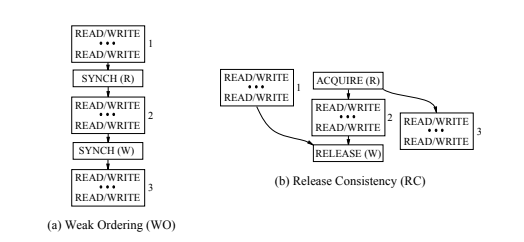
\includegraphics[width=0.9\textwidth]{figures/compare.png}
  \label{Fig:weak}
\end{figure}

\end{frame}





\begin{frame}
	\frametitle{Release Consistency Model}
Release Consistency ist sichergestellt, wenn:
	\begin{itemize}
\bigskip
		
		\item Alle 'aquire'-Operationen durchlaufen sind, bevor geschrieben oder gelesen wird \bigskip
		\item Alle Schreib- oder Leseoperationen durchlaufen sind, bevor 'release' startet \bigskip
		\item Alle Schreiboperationen von A von B gesehen werden, nachdem A sie released hat und bevor B sie aquired hat 

	\end{itemize}


\end{frame}
\note{\newline \newline Release Consistency ist sicher gestellt wenn 
\newline \newline Alle Schreiboperationen von A von B gesehen werden, nachdem A sie released hat und bevor B sie aquired hat
		\newline \newline Alle 'aquire'-Operationen durchlaufen sind, bevor geschrieben oder gelesen wird 
		\newline \newline Alle Schreib- oder Leseoperationen durchlaufen sind, bevor 'release' startet
\newline \newline Die nächste Abbildung verdeutlicht das
} 


\begin{frame}
	\frametitle{Release Consistency Model}
\begin{figure}[htbp] 
  \centering
  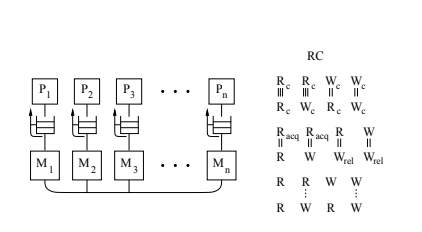
\includegraphics[width=0.9\textwidth]{figures/rc.png}
  \label{Fig:weak}
\end{figure}

\end{frame}



\begin{frame}
	\frametitle{Release Consistency Model}
	\begin{itemize}

		\item Release muss auf vorangegange Operationen warten \bigskip
		\item Aquire muss nicht auf vorangegangene Operationen warten \bigskip
		\item Folgende Operationen warten  nicht auf Fertigstellung von Release \bigskip
		\item Folgende Operationen warten auf Fertigstellung von Aquire \bigskip
	\end{itemize}
\end{frame}
\note{
\newline \newline Release muss auf vorangegange Operationen warten
\newline \newline Aquire muss nicht auf vorangegangene Operationen warten
\newline \newline Folgende Operationen warten  nicht auf Fertigstellung von Release
\newline \newline Folgende Operationen warten auf Fertigstellung von Aquire
}

\begin{frame}
	\frametitle{Release Consistency Model}
	\begin{itemize}


		\item Mehr Flexibilität und Schnelligkeit zwischen ’acquire’ und ’release’ \bigskip
		\item Operationen überlappbar \bigskip
\end{itemize}
\begin{itemize}
		\item Es gibt insgesamt mehr Operationen  \bigskip
		\item Mehr Operationen müssen ausgeführt und geplant werden 

		

	\end{itemize}


\end{frame}
\note{\newline \newline Vorteile

\newline \newline Das Ergebnis sind mehr Flexibilität und Schnelligkeit zwischen ’acquire’ und ’release’
\newline \newline Operationen überlappbar
\newline \newline Nachteile
\newline \newline es  gibt insgesamt mehr Operationen
\newline \newline Mehr Operationen müssen ausgeführt und geplant werden 
}


%%%%%%%%%%%%%%%%%%%%

\section{Gegenüberstellung}
\begin{frame}{Gliederung}
   
    	\tableofcontents[currentsection, subsectionstyle=show/show/hide]
 	%\sectionframe	
	%\subsectionframe
\end{frame}

\begin{frame}
	\frametitle{Gegenüberstellung}
\begin{figure}[htbp] 
  \centering
  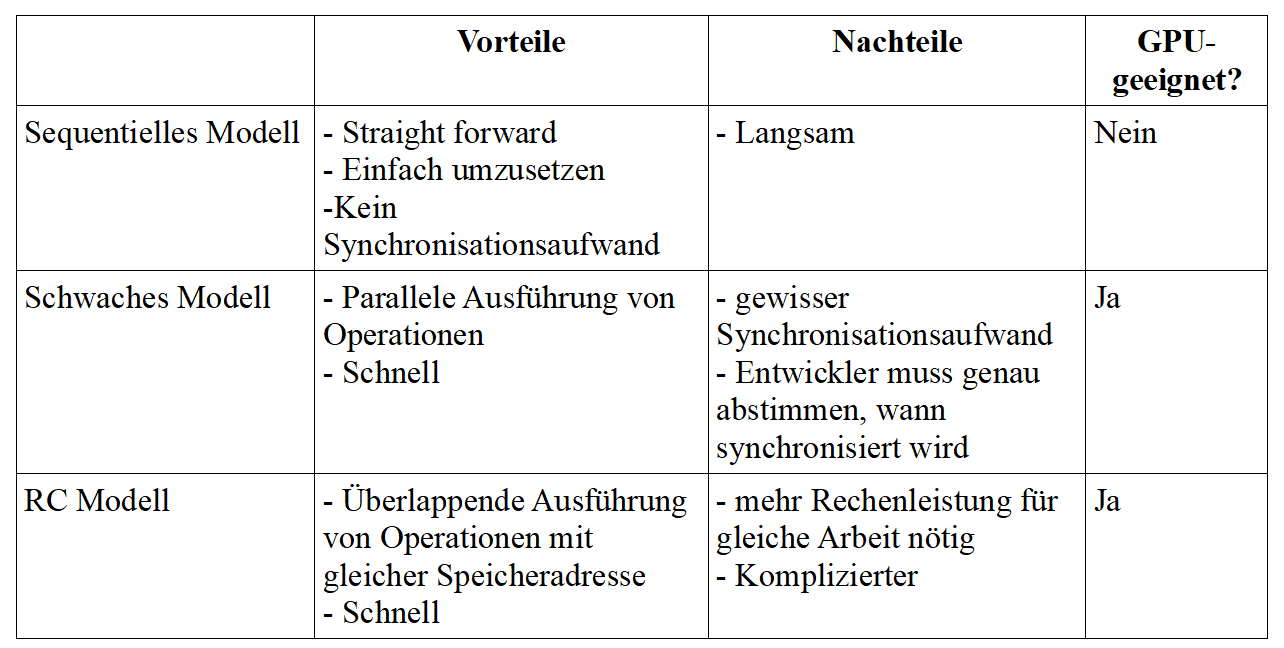
\includegraphics[width=0.9\textwidth]{figures/vergleich.png}
  \label{Fig:vg}
\end{figure}

\end{frame}

\section{Andere Ansätze}

\begin{frame}{Gliederung}
   
    	\tableofcontents[currentsection, subsectionstyle=show/show/hide]
 	%\sectionframe	
	%\subsectionframe
\end{frame}


\begin{frame}
	\frametitle{CUDA und OpenCL}
		\begin{itemize}

		\item GPUPU Programmiermodelle \bigskip
		\item Fokus auf Optimierung datenparalleler Entwicklung \bigskip
		\item Mehrere Threads sollen auf dieselbe Speicheradresse zugreifen können \bigskip
		\item CUDA basiert auf Schwachem Konsistenzmodell \bigskip
		\item OpenCL basiert auf RC-Modell \bigskip
		\item Bieten Framework, um diese Zugriffe für den Programmierer zu vereinfachen \bigskip
		\item OpenCL über Api-Zugriffe, CUDA über C-Entwicklung

\bigksip
\item Heute gängige implementierte Form zur Speicherverwaltung

	\end{itemize}
\end{frame}
\note{\newline \newline GPUPU Programmiermodelle 
		\newline \newline Fokus auf Optimierung datenparalleler Entwicklung 
		\newline \newline Mehrere Threads sollen auf dieselbe Speicheradresse zugreifen können 
		\newline \newline CUDA basiert auf Schwachem Konsistenzmodell 
		\newline \newline OpenCL basiert auf RC-Modell 
		\newline \newline Bieten Framework, um diese Zugriffe für den Programmierer zu vereinfachen
		\newline \newline OpenCL über Api-Zugriffe, CUDA über C-Entwicklung
\newline \newline Heute gängige implementierte Form zur Speicherverwaltung
}

\section{Fazit}
\begin{frame}{Gliederung}
   
    	\tableofcontents[currentsection, subsectionstyle=show/show/hide]
 	%\sectionframe	
	%\subsectionframe
\end{frame}

\begin{frame}
	\frametitle{Fazit}
\begin{itemize}

		\item Es gibt viele Modelle, die unterschiedliche Zwecke erfüllen \bigskip
		\item Gut für GPUs: Modelle, die auf Performance und Datenparallelität ausgerichtet sind \bigskip
		\item Weak Consistency und Release Consistency Model guter Ansatz\bigskip
		\item CUDA und OpenCL bieten Framework und optimierte Modelle  \bigskip
		\item Bauen auf den vorgestellten Modellen auf \bigskip
		\item Je nach Bedürfnis CUDA oder OpenCL verwenden


	\end{itemize}
\end{frame}
\note{\newline \newline Es gibt viele Modelle, die unterschiedliche Zwecke erfüllen 
		\newline \newline Gut für GPUs: Modelle, die auf Performance und Datenparallelität ausgerichtet sind 
		\newline \newline Es ist zu beachten, dass es CPU MOdelle sind, deshalb Weak Consistency und Release Consistency Model guter Ansatz
		\newline \newline CUDA und OpenCL bieten Framework und optimierte Modelle  
		\newline \newline Bauen auf den vorgestellten Modellen auf 
		\newline \newline Je nach Bedürfnis CUDA oder OpenCL verwenden
}

\begin{frame}
	
Vielen Dank für Ihre Aufmerksamkeit!
\end{frame}


\end{document}

